\documentclass[12pt,a4paper]{article}

\usepackage[margin=1in]{geometry}
\usepackage{graphicx}
\usepackage{xcolor}
\usepackage{array}
\usepackage{tikz}
\usepackage{float}
\usepackage{hyperref}
\usepackage{enumitem}

\usetikzlibrary{arrows.meta, positioning, shapes.geometric, fit}

\hypersetup{
    colorlinks=true,
    linkcolor=blue,
    urlcolor=blue
}

\definecolor{boxblue}{RGB}{224,240,255}
\definecolor{boxgreen}{RGB}{226,247,232}
\definecolor{boxyellow}{RGB}{255,245,204}
\definecolor{boxred}{RGB}{255,229,229}
\definecolor{linegray}{RGB}{80,90,105}

\title{\textbf{Snake Game with Human and Q-Learning AI Modes}}
\author{Mini Project Report}
\date{}

\begin{document}

\maketitle

\section{Introduction}

This project implements a classic grid-based Snake Game with two modes: Human Mode and AI Mode. In Human Mode, the user controls the snake using keyboard or on-screen buttons. In AI Mode, the snake plays automatically using Q-Learning, a reinforcement learning technique. The project demonstrates how an agent can learn actions based on rewards, penalties, and repeated gameplay episodes.

\section{Problem / Application Description}

The objective is to build a Snake Game that supports both manual gameplay and autonomous AI gameplay. The snake must move around a grid, eat randomly spawned food, grow in length, avoid wall collisions, and avoid colliding with itself. The AI agent learns to play by interacting with the game environment and updating a Q-table based on rewards.

\section{System Overview}

The system has two main user-facing modes. The browser version provides buttons for mode selection, restart, speed control, and directional control. The Python version uses Pygame for desktop gameplay. Both versions follow the same core Snake Game rules.

\subsection{Architecture Diagram}

\begin{figure}[H]
\centering
\resizebox{\textwidth}{!}{
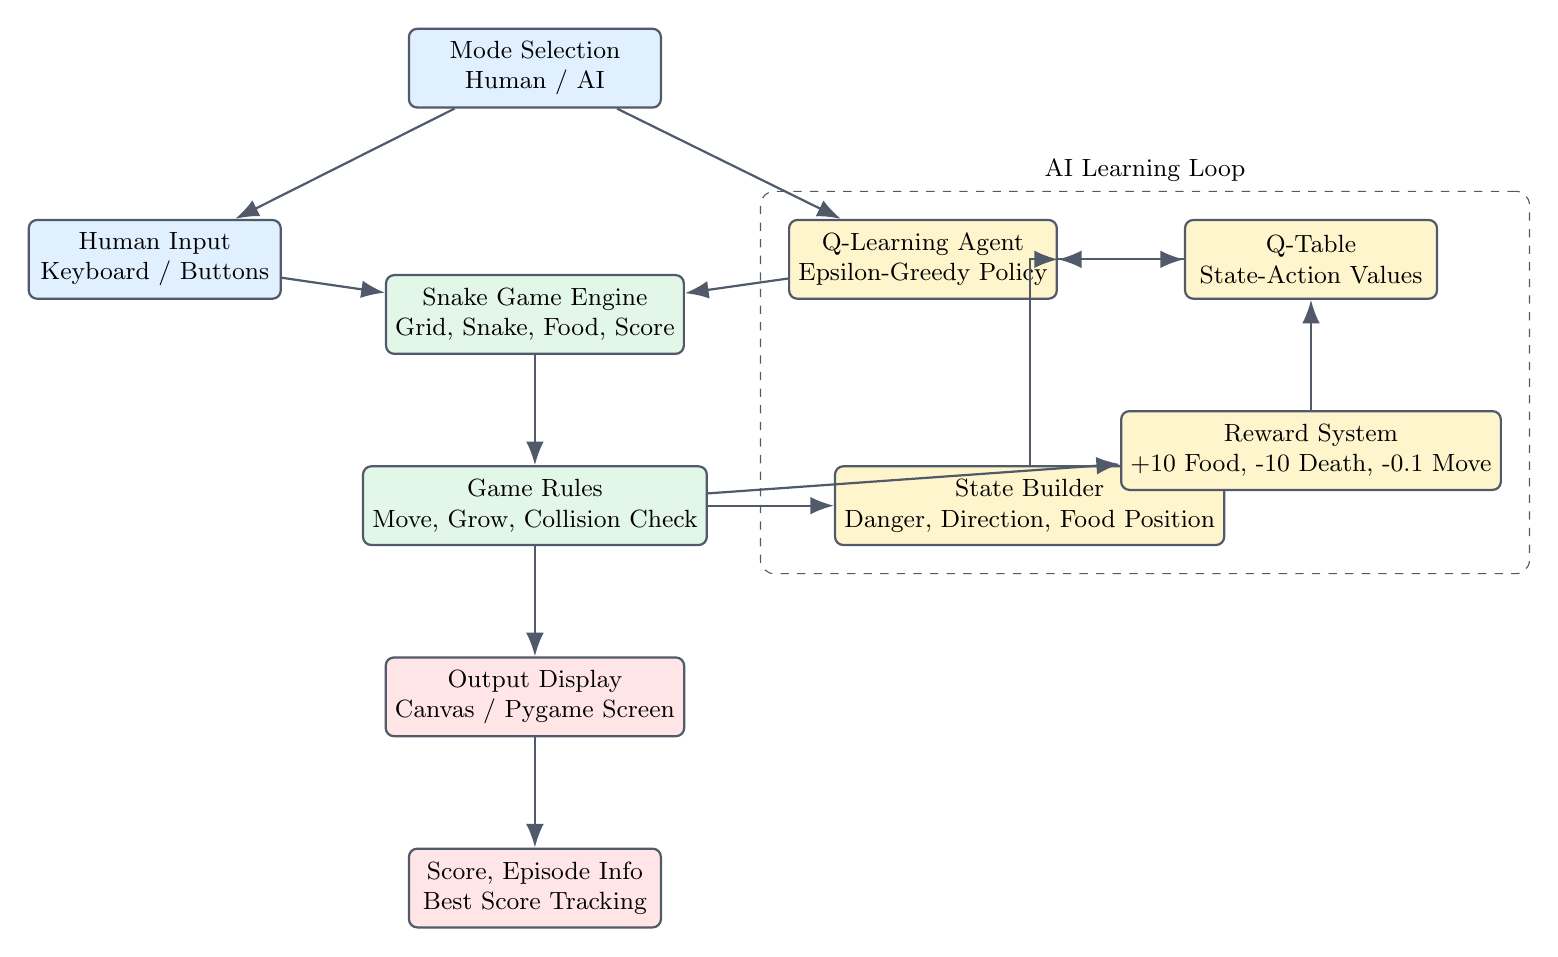
\begin{tikzpicture}[
    node distance=1.4cm and 1.6cm,
    box/.style={
        rectangle,
        rounded corners=3pt,
        draw=linegray,
        thick,
        align=center,
        minimum width=3.2cm,
        minimum height=1cm,
        font=\small
    },
    userbox/.style={box, fill=boxblue},
    gamebox/.style={box, fill=boxgreen},
    aibox/.style={box, fill=boxyellow},
    outbox/.style={box, fill=boxred},
    arrow/.style={-{Latex[length=3mm]}, thick, draw=linegray}
]

\node[userbox] (menu) {Mode Selection\\Human / AI};

\node[userbox, below left=of menu] (human) {Human Input\\Keyboard / Buttons};
\node[aibox, below right=of menu] (agent) {Q-Learning Agent\\Epsilon-Greedy Policy};

\node[gamebox, below=2.1cm of menu] (engine) {Snake Game Engine\\Grid, Snake, Food, Score};
\node[gamebox, below=of engine] (rules) {Game Rules\\Move, Grow, Collision Check};

\node[aibox, right=of rules] (state) {State Builder\\Danger, Direction, Food Position};
\node[aibox, right=of agent] (qtable) {Q-Table\\State-Action Values};
\node[aibox, below=of qtable] (reward) {Reward System\\+10 Food, -10 Death, -0.1 Move};

\node[outbox, below=of rules] (render) {Output Display\\Canvas / Pygame Screen};
\node[outbox, below=of render] (result) {Score, Episode Info\\Best Score Tracking};

\draw[arrow] (menu) -- (human);
\draw[arrow] (menu) -- (agent);
\draw[arrow] (human) -- (engine);
\draw[arrow] (agent) -- (engine);
\draw[arrow] (engine) -- (rules);
\draw[arrow] (rules) -- (render);
\draw[arrow] (render) -- (result);

\draw[arrow] (rules) -- (state);
\draw[arrow] (state) |- (agent);
\draw[arrow] (agent) -- (qtable);
\draw[arrow] (reward) -- (qtable);
\draw[arrow] (rules) -- (reward);
\draw[arrow] (qtable) -- (agent);

\node[draw=linegray, dashed, rounded corners=5pt, fit=(agent) (qtable) (reward) (state), inner sep=0.35cm, label={[font=\small]above:AI Learning Loop}] {};

\end{tikzpicture}
}
\caption{Architecture diagram of the Snake Game with Human and Q-Learning AI modes.}
\end{figure}

\subsection{Workflow: Input -- Processing -- Output}

\begin{enumerate}[label=\arabic*.]
    \item The user selects Human Mode or AI Mode.
    \item In Human Mode, keyboard or button input controls the snake direction.
    \item In AI Mode, the Q-learning agent selects an action: straight, left, or right.
    \item The game engine updates the snake position, food state, score, and collision status.
    \item The reward system gives positive or negative feedback to the AI.
    \item The Q-table is updated using the Q-learning formula.
    \item The updated game state is rendered on the screen.
\end{enumerate}

\section{AI Technique Used}

\subsection{Technique Name}

Q-Learning Reinforcement Learning

\subsection{Description}

Q-Learning is a model-free reinforcement learning algorithm. The agent learns the value of actions in different states by repeatedly interacting with the environment. In this project, the AI observes danger around the snake, the current direction, and the food position. Based on this state, it chooses one of three actions: go straight, turn left, or turn right.

\subsection{State Representation}

The state includes:

\begin{itemize}
    \item Danger straight
    \item Danger left
    \item Danger right
    \item Current movement direction
    \item Food position relative to the snake head
\end{itemize}

\subsection{Actions}

\begin{itemize}
    \item Straight
    \item Left
    \item Right
\end{itemize}

\subsection{Rewards}

\begin{itemize}
    \item Eat food: $+10$
    \item Death: $-10$
    \item Each move: $-0.1$
\end{itemize}

\subsection{Justification}

Q-Learning is suitable for this project because Snake can be represented as a sequence of states, actions, and rewards. The agent does not need a predefined path. Instead, it improves by playing multiple episodes and learning which actions produce better long-term scores.

\section{Technology Stack}

\begin{table}[H]
\centering
\renewcommand{\arraystretch}{1.35}
\begin{tabular}{|p{0.32\textwidth}|p{0.55\textwidth}|}
\hline
\textbf{Component} & \textbf{Tools Used} \\
\hline
Frontend & HTML, CSS, JavaScript, Canvas, Buttons, Keyboard Controls \\
\hline
Desktop UI & Python, Pygame \\
\hline
AI Libraries & NumPy, Q-table Dictionary / Browser Local Storage \\
\hline
Game Logic & Grid-based Snake Engine, Collision Detection, Random Food Spawning \\
\hline
Storage & Pickle file for Python Q-table, Local Storage for browser Q-table \\
\hline
Deployment & Local browser execution using \texttt{index.html} \\
\hline
\end{tabular}
\caption{Technology stack used in the Snake Game project.}
\end{table}

\section{Results / Output}

The completed project provides:

\begin{itemize}
    \item A playable Human Mode with real-time snake movement.
    \item An AI Mode where the snake plays automatically using Q-Learning.
    \item Score display and best score tracking.
    \item Episode information printed during AI training.
    \item A website interface with buttons for Human Mode, AI Mode, Restart, Speed Control, and Direction Control.
\end{itemize}

\section{Application Link}

Drive Link: \underline{\hspace{10cm}}

\section{Source Code Link}

Drive/GitHub Link: \underline{\hspace{9cm}}

\end{document}
